\documentclass[sigconf]{acmart}

\usepackage{booktabs} % For formal tables


% Copyright
%\setcopyright{none}
%\setcopyright{acmcopyright}
%\setcopyright{acmlicensed}
\setcopyright{rightsretained}
%\setcopyright{usgov}
%\setcopyright{usgovmixed}
%\setcopyright{cagov}
%\setcopyright{cagovmixed}


% DOI
\acmDOI{10.xxx/xxx_x}

% ISBN
\acmISBN{123-4567-24-567/08/06}

%Conference
\acmConference[MANLANG'17]{International Conference on Managed Languages \& Runtimes}{July 2017}{Prague, Czech Republic} 
\acmYear{2017}
\copyrightyear{2017}

\acmPrice{15.00}


\begin{document}
\title{Flexible Object Layout Evolution on Hosted Dynamic Language Runtime}
%\titlenote{Produces the permission block, and copyright information}
%\subtitle{Extended Abstract}
%\subtitlenote{The full version of the author's guide is available as
%  \texttt{acmart.pdf} document}


\author{Wei Zhang}
\affiliation{%
  \institution{Facebook, Inc.}
  \streetaddress{1 Hacker way}
  \city{Menlo Park} 
  \state{California} 
  \postcode{94025}
}
\email{zwei@fb.com}

\author{Stefan Brunthaler}
\affiliation{%
  \institution{Paderborn University}
  \streetaddress{Warburger Stra{\ss}e 100}
  \city{Paderborn} 
  \state{Germany} 
  \postcode{33098}
}
\email{s.brunthaler@upd.de}

\author{Michael Franz}
\affiliation{%
  \institution{University of California, Irvine}
  \city{Irvine} 
  \state{California} 
  \postcode{92697}
}
\email{franz@uci.edu}


\begin{abstract}
Python is an object oriented programing language.
It is a common practice for programmers to encapsulate state and logic using classes in Python programs.
As an implementation of the Python language, it is essential for us to ensure the performance of object operations and method calls in ZipPy.
\end{abstract}

%
% The code below should be generated by the tool at
% http://dl.acm.org/ccs.cfm
% Please copy and paste the code instead of the example below. 
%
\begin{CCSXML}
<ccs2012>
 <concept>
  <concept_id>10010520.10010553.10010562</concept_id>
  <concept_desc>Computer systems organization~Embedded systems</concept_desc>
  <concept_significance>500</concept_significance>
 </concept>
 <concept>
  <concept_id>10010520.10010575.10010755</concept_id>
  <concept_desc>Computer systems organization~Redundancy</concept_desc>
  <concept_significance>300</concept_significance>
 </concept>
 <concept>
  <concept_id>10010520.10010553.10010554</concept_id>
  <concept_desc>Computer systems organization~Robotics</concept_desc>
  <concept_significance>100</concept_significance>
 </concept>
 <concept>
  <concept_id>10003033.10003083.10003095</concept_id>
  <concept_desc>Networks~Network reliability</concept_desc>
  <concept_significance>100</concept_significance>
 </concept>
</ccs2012>  
\end{CCSXML}

\ccsdesc[500]{Computer systems organization~Embedded systems}
\ccsdesc[300]{Computer systems organization~Redundancy}
\ccsdesc{Computer systems organization~Robotics}
\ccsdesc[100]{Networks~Network reliability}


\keywords{ACM proceedings, \LaTeX, text tagging}


\maketitle

\section{Introduction}

% object model is critical
All data is presented as object in mainstream dynamic languages like Python, Ruby and JavaScript.
Programs written in those languages interact with data using objects.
Object model, the implementation behind the object representation is a core component of a language runtime implementation.
Not only it has to be efficient for accessing the reperesented data, it also needs to respect the dynamic nature of those languages.
An efficient dynamic language implementation should handled object modifications at runtime in less expensive ways.

% hosted language is the trend
Despite their popularity, performance has been the weakness of dynamic languages.
Languages like Python and Ruby are originally implemented as interpreters.
Although interpreters are easy to implement, their performance is suboptimal.
To address this weakness, we have seen previous works that have improved the performance of dynamic languages
by constructing a complete just-in-time (JIT) compilation based virtual machine for one particular language.
This approach offers promising performance benefit, but incurs significant implementation costs.

Alternatively, language implementors can build their languages on top of an existing mature virtual machine such as the Java Virtual machine (JVM).
In this way, the ``guest'' language can reuse the existing components of the ``hosting'' virtual machine to alleviate its implementation costs.
It also provide the opportunity for the ``hosted'' language to take advantage of the underlying JIT compiler to address its performance issue.
We explore the performance potential of ``hosted'' interpreters for dynamic languages.
We do so by hosting a ``highly dynamic'' language (Python) on the JVM, a VM for ``moderately dynamic'' languages.

% existing hosted object model has drawbacks
We found that existing hosted dynamic languages have not addressed their object model in an efficient way.
Jython, a JVM based Python implementation replicate the same object model design we saw in CPython to Java.
This approach failed to identify the strength of the underlying VM.
It relies on the assumption that the underlying JIT is powerful enough to optimize any type of program.
Truffle's object model framwork provided an efficient way for guest langauge developer to quickly build a performant object model.
It makes use of highly efficient constructs provided by the ``hosting'' VM.
However it's design uses a fixed object storage layout, which often trades space for performance.
In practice, this approach puts undesired pressure onto the garbage collector when running programs allocating a large number of objects.

% our extension to that
In this paper, we propose an improved object model for hosted dynamic languages.
It addresses the performance and space drawbacks of the existing works.
We demonstrate our technique using our own full-fledged prototype implementation of Python 3, called ZipPy\footnote{Publicly available at \url{https://bitbucket.org/ssllab/zippy}}, which targets the Java virtual machine (JVM).
ZipPy uses the Truffle framework to optimize interpreted programs in stages, first collecting type feedback in the AST interpreter, then just-in-time compiling an AST down to optimized machine code.

\noindent{}Our contributions are:

\begin{itemize}

\item We present an efficient object model implementation for hosted dynamic languages.

\item We introduce \emph{flexible object layout evolution}, a new technique our system uses to minimize space overheads incurred by object model.

\item We provide results of a careful and detailed evaluation of our optimization and report:
  \begin{itemize}
  \item an average saving of xxx over the fixed storage baseline.
  \end{itemize}
\end{itemize}

\section{Background}

In Python all data is an object.
CPython, the original implementation of Python, constructs every data type in Python as a heap allocated data structure.
Since it is written in C, CPython implements Python built-in data types using C struct and user defined types using hash maps.
This model results in expensive arithmetic operations due to frequent accesses and allocations of data structures in the heap.
Hash map based object model is also inefficient.
Although the cost of hash map operations is amortized for large data sets, the overhead of retrieving or updating a single map entry is still expensive.
In a hash map based object model, retrieving the value of an object field, or an object attribute in Python, is equivalent to reading the value of a map entry.
This operation involves a hashing calculation and a few steps of memory accesses before reaching the memory address that stores the target value.
On the other hand, in a traditional programming language like Java, an object field access, if optimized, is simply a single memory read.
In summary, object model inefficiency is the main impediment to the performance of popular dynamic languages like Python.

\subsection{Jython's Object Model Design}

Existing JVM based Python implementations like Jython, however, replicate the same object model design we saw in CPython.
The main approach they took is porting the existing design from C to Java hoping that the underlying Java compiler will magically optimize it.
This approach failed to realize that, although, the Java JIT compiler is powerful, its strength is in compiling and optimizing programs written in Java,
the first class citizen of the JVM.
Hence, without additional knowledge to the guest language, the Java compiler is unable to address the miss match between the object model of the guest language and Java in an efficient way.
A more efficient solution requires identifying the strengths of the Java compiler and mapping critical components of the guest language onto efficient constructs offered of the JVM.
In the rest of this Section, we describe how we close the gap between the object models of Python and the JVM in ZipPy.

\subsection{Python on Truffle}

\begin{figure*}[!ht]
\centering
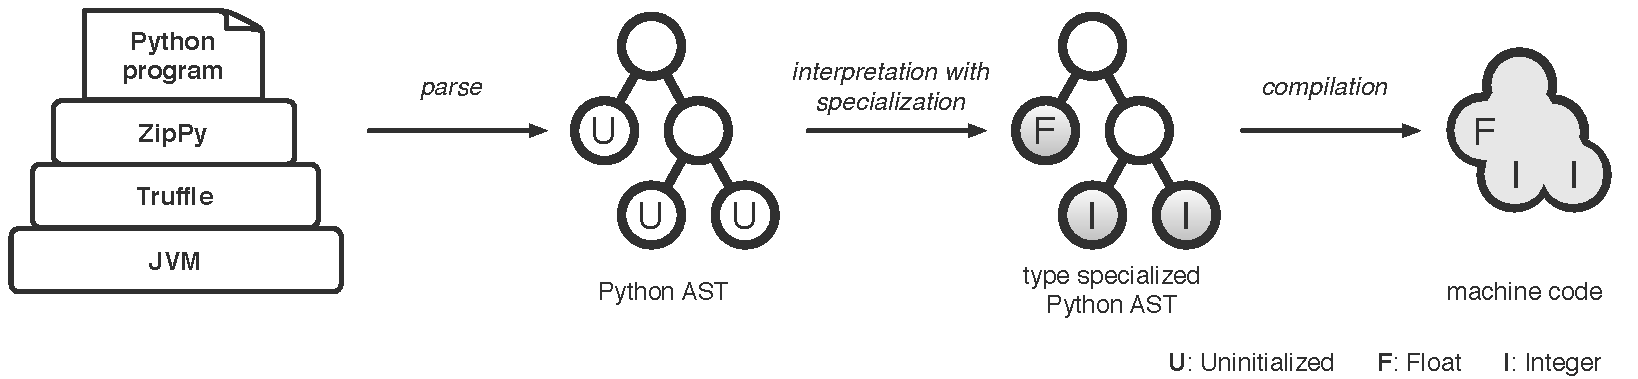
\includegraphics[scale=0.50]{figures/python-on-truffle.pdf}
\caption{Python on Truffle}
\label{fig:python_on_truffle}
\end{figure*}

In principle, ``everything'' can change at any moment in dynamic language programs.
This dynamic nature is the major impediment to ahead-of-time optimization.
In practice, however, programmers tend to minimize the rate of change, which makes the code highly predictable.
Types, for instance, typically remain stable between successive executions of a particular operation instance.
Deutsch and Schiffman report that speculative type specialization succeeds 95\% of the time in their classic Smalltalk-80 implementation~\cite{Deutsch1984}.

Truffle is a self-optimizing runtime system that makes it easy to perform type specialization for dynamic languages running on top of the Java Virtual Machines (JVM)~\cite{Wurthinger+13}.
It allows language implementers to implement their guest language by writing an AST interpreter using Java.
An interpreter written in this way enjoys low cost type specialization via automatic node rewriting~\cite{Wurthinger+12,Brunthaler2010inca,Brunthaler2010quickening}.
AST node rewriting collects runtime type information, and speculatively replaces the existing nodes with specialized and more efficient ones.
Subsequently, Truffle just-in-time compiles the specialized AST, written in Java, directly to machine code using the underlying Java compiler.
Upon a type mis-speculation, the specialized AST node handles the type change by replacing itself with a more generic one.
The node replacement triggers deoptimization from the compiled code and transfers execution back to the interpreter.
If the re-specialized AST stays stable, Truffle can again compile it to machine code.

Our system, ZipPy, is a full-fledged prototype Python 3 implementation built atop Truffle.
It leverages Truffle's type specialization feature and its underlying compilation infrastructure (see Figure~\ref{fig:python_on_truffle}).
This architecture helps ZipPy outperform Python implementations that either do not exploit runtime type specialization or lack a just-in-time compiler.
However, Truffle has no knowledge about specific high level guest language semantics, like generators in Python.
Further performance exploration of a guest language will mainly benefit from better insights on distinct features of the language and making better use of the host compiler based on those insights.
In this paper we focus on guest language level optimizations we added to ZipPy.

\section{ZipPy's Object Model Design}

\begin{figure}
\centering
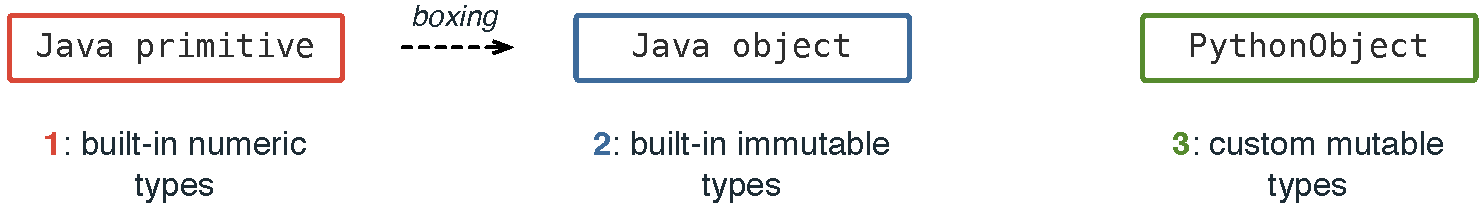
\includegraphics[scale=.34]{figures/three-data-representations}
\caption{Three data representations for Python objects}
\label{fig:three-data-representations}
\end{figure}

Python, although being a dynamic language, has a rich set of built-in types that are backed by C structs.
These types are inherently immutable.
Meaning that Python programs cannot add or remove attributes to or from it at runtime.
This feature separates it from languages like Ruby where you can monkey patch core classes of the language.
But it does offer opportunities for the language implementations like ZipPy to model immutable built-in types in a more efficient way.
Custom types defined in Python level are dynamic and mutable.
They can be as expected manipulated as map or dictionaries at runtime.
In the rest of this Section, we explain how we model them efficiently in ZipPy.

Python does offer more advanced features like metaclasses and attribute access customizations.
They do make the use of the language even more dynamic.
However, in this paper we donot focus on those advanced features.

\subsection{Multiple Data Representations}

ZipPy internally uses multiple data representations to model Python objects.
Figure~\ref{fig:three-data-representations} illustrates this design scheme.
The descriptions of each data representation are as follows:

\begin{enumerate}

\item \textbf{Built-in numeric types}
ZipPy, as explained in Chapter~, models some built-in numeric types, like \texttt{bool}, \texttt{int} and \texttt{float}, using Java primitives.
This approach helps to achieve Java level performance for arithmetic operations in ZipPy.
We refer types that has a Java primitive representation as \emph{unboxable}.
Each \emph{unboxable} numeric type in ZipPy has a corresponding \emph{boxed} representation using Java objects as a fall-back.
As shown in the Figure, a boxing operation will convert an instance of unboxable type, e.g., \texttt{int}, from its Java primitive representation to the boxed one.

\item \textbf{Built-in immutable types}
Similar to Jython, we implement Python built-in types including numeric types as regular Java classes.
In this way we map Python's built-in type hierarchy onto a Java class based type hierarchy.
Unlike custom types, all built-in types in Python are immutable meaning that user program cannot modify the attributes of an instance of a built-in type.
We take advantage of this immutability by modeling Python built-in types directly using Java classes on the JVM.

\item \textbf{Custom mutable types}
All custom or user defined types in Python are mutable.
That includes Python modules, custom type definitions written in Python and instances of custom classes.
We model them using still a regular Java object, an instance of \texttt{PythonObject} in ZipPy, to circumvent the performance overhead incurred by using a hash map.
ZipPy maps Python attribute accesses to field accesses on the \texttt{PythonObject} object.
We support attribute modifications by maintaining an object layout table for each Python object.
The object layout table keeps track of the memory offset for each attribute that is currently stored on the object.
We will discuss how we support attribute modifications on custom types in more detail in Section~.

\end{enumerate}

Although we model Python objects using different physical data representations, our approach preserve the semantics that every data in Python is an object.
ZipPy support object like operations on each of the data representations described above.
What differs our approach to the existing ones is that we do not treat all Python data types in the same way.
We try to pick the most efficient construct offered by the JVM that is suitable for implementing particular types in Python.
To be more specific, modeling Python numbers as Java primitives enables the best arithmetics performance achievable on the JVM.
Using Java object to model Python object brings the opportunity for ZipPy to close the performance gap of object operations between existing implementations of Python and Java.

\subsection{Modeling Custom Mutable Types}
\label{sec:ch5-custom-mutable-types}

\begin{figure}
\centering
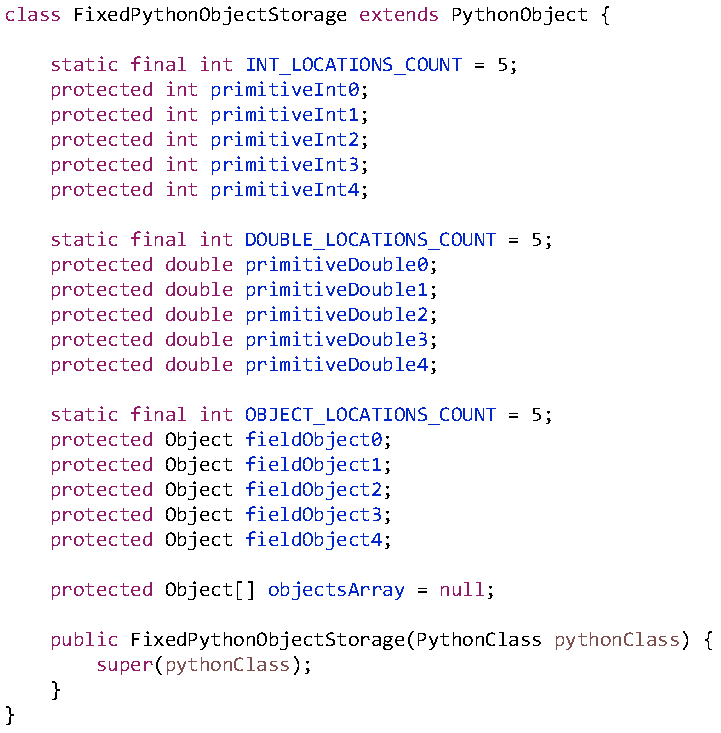
\includegraphics[scale=.7]{figures/fixed-python-object-code}
\caption{The implementation of \texttt{PythonObject}}
\label{ch5-fixed-python-object-code}
\end{figure}

\begin{figure}
\centering
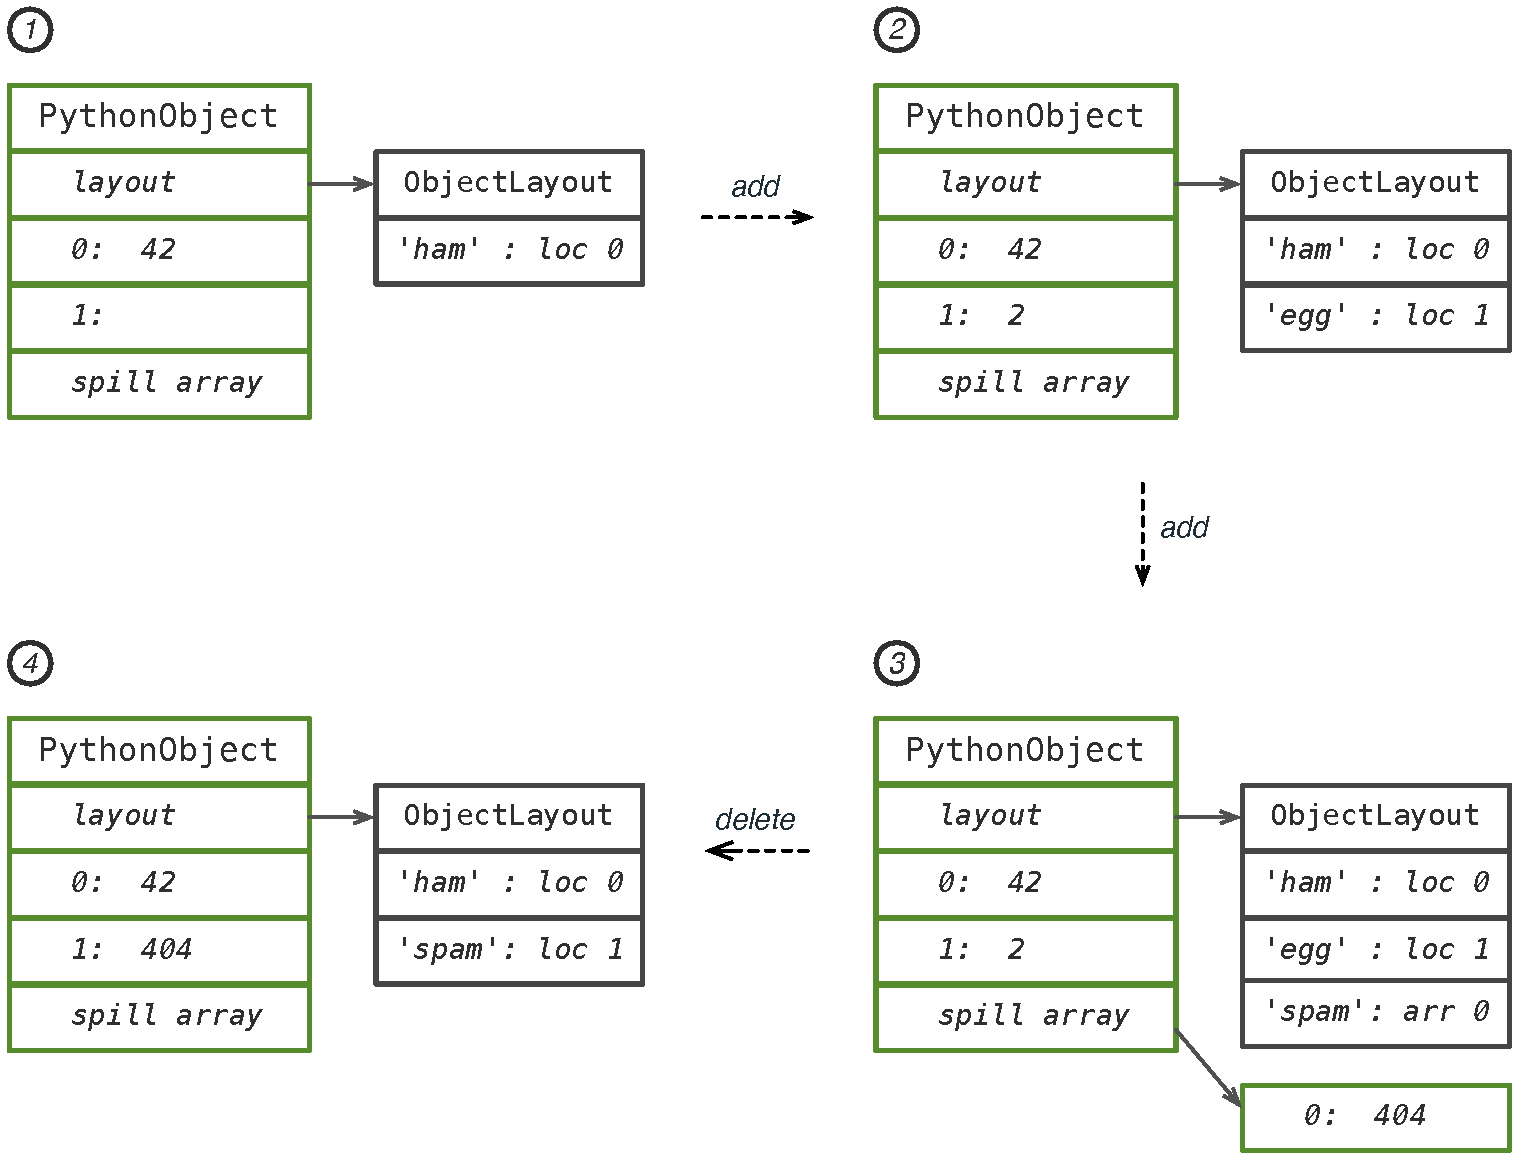
\includegraphics[scale=.34]{figures/mutable-object-layout-change}
\caption{Mutable object layout}
\label{ch5-mutable-object-layout-change}
\end{figure}

Python allows programmers to add, modify or delete attributes on an object during the execution of the program.
On the other hand, a Java object is fixed.
You can modify the value of a field, but cannot resize or change the layout of an object.
We support this dynamic feature of Python by implementing each Python object using a combination of a fixed \texttt{PythonObject} and a re-sizable object layout.

Figure~\ref{ch5-fixed-python-object-code} shows an implementation of \texttt{PythonObject} in ZipPy.
Each \texttt{PythonObject} has a fixed number of fields of both primitive and reference types to accommodate its attributes.
Each field on the object is a \emph{location}.
The object stores each of its attribute on a dedicated \emph{location}.
ZipPy tries to store an unboxed attribute in an unboxed location to avoid the overhead of boxing.
For instance, it tries to store a Java \texttt{int} in an \texttt{int} field when possible.
If all \texttt{int} fields are taken, it tries to stores the attribute in an \emph{boxed} location or an object field.
If no in-object location is available anymore (taken by other attributes), ZipPy will spill the incoming attribute to be stored in the additional object array (field \texttt{objectArray} in Figure~\ref{ch5-fixed-python-object-code}).
The additional object array gives the fixed \texttt{PythonObject} the ability to store more attributes than its own capacity by paying the price of another level of direction and possibly auto-boxing.

An object layout attached to a \texttt{PythonObject} keeps track of the list of attributes stored on the object as well as the location of each attribute.
It is essentially a table that maps the symbol of an attribute to its location.
The table records modifications made dynamically to the attributes of the object.
Figure~\ref{ch5-mutable-object-layout-change} illustrates how this process works by using a hypothetical Python object.
The layout of the shown object goes through the following stages:

\begin{enumerate}

\item The object initially has one attribute \textsf{ham} stored in location $0$ with the value $42$.

\item After adding the attribute \textsf{egg}, the object now has both \textsf{ham} and \textsf{egg} stored in location $0$ and $1$ respectively.

\item Since both in-object locations are taken, the object stores the new attribute \textsf{spam} in the spill array at the index $0$.
The rest of the layout remain unchanged.

\item The deletion of \textsf{egg} frees location $1$ on the object.
The object reassigns the newly available in-object location to \textsf{spam} to make sure that location assignments are optimal.
It also update the layout table to reflect the new changes.

\end{enumerate}

We simplified the structure of the Python object shown in Figure~\ref{ch5-mutable-object-layout-change} for brevity.
The actual algorithm for a layout update is more complicated.
Adding or deleting an attribute triggers a layout update.
The layout update tries to stores as many unboxed attributes in an unboxed location as possible.
The spill array allocation is lazy so that we only allocate the array when necessary.
During the layout update, ZipPy calculates the size of the additional spill array needed to accommodate all the attributes.
If it requires a spill array, we conservatively allocate an array that is just enough to store all the attributes.

In Python, attribute types can change at runtime.
An attribute type change also triggers a layout update.
Our current solution to handle such a type change is to assign a location that matches the most generic type of the attribute.
Once an unboxed attribute becomes boxed, we always assign a boxed location for this attribute in the future.

Our approach uses \texttt{PythonObject}s simply as a physical storage for the attributes of a Python object.
We detach the layout description of the Python object from its storage component.
This approach gives us the freedom to customize the behavior of attribute accesses in ZipPy without being restricted by Java's own object model.
Since we model class objects in the same way as we do for regular objects in Python, they enjoy the same potential performance benefit achieved by this design.

\subsection{Inline Caching for Attribute Accesses}

As explained in Section~\ref{sec:ch5-custom-mutable-types}, the layout table stores the location of object attributes.
Accessing an attribute requires looking up its location information from the layout table and then performing a memory read or write at the obtained memory location.
Since we implement the layout table using a hash map, the cost of accessing the table is as expensive as attribute accesses on a hash map based object.
However, ZipPy optimizes attribute accesses by caching attribute locations after a full layout table lookup.
This technique, inspired by previous research on virtual machines~\cite{Deutsch1984, Holzle+1991, Brunthaler2010inca}, amortizes the cost of accessing the same attribute on the Python objects of the same type.

\subsubsection{Attribute Access Dispatch Chain}
\label{sec:ch5-attribute-access-dispatch-chain}

\begin{figure}
\centering
\subfigure[Structure of \texttt{GetAttributeNode}]{
  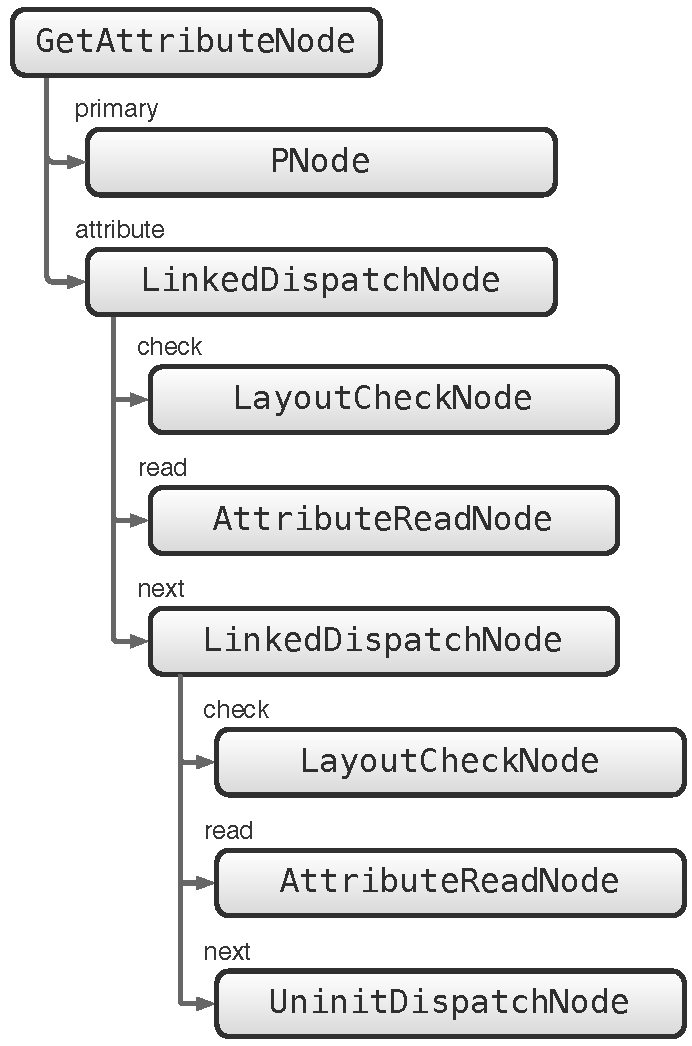
\includegraphics[scale=.4]{figures/get-attribute-node}
  \label{fig:ch5-get-attribute-node}
}
\subfigure[Structure of \texttt{SetAttributeNode}]{
  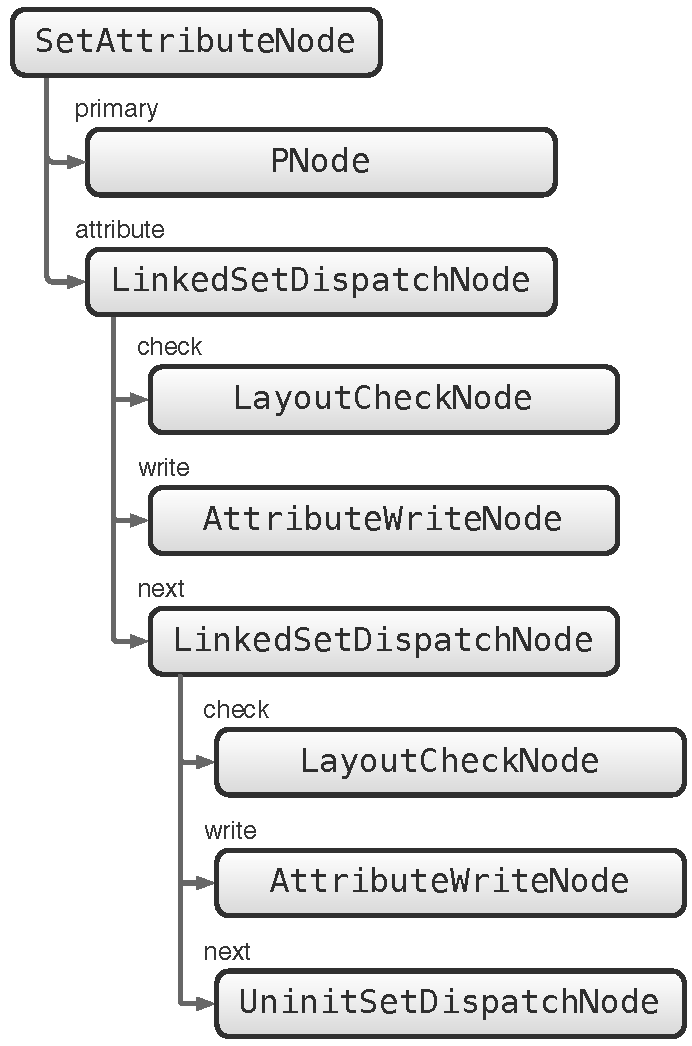
\includegraphics[scale=.4]{figures/set-attribute-node}
  \label{fig:ch5-set-attribute-node}
}
\caption{Attribute access dispatch chain}
\label{fig:ch5-attribute-access-dispatch-chain}
\end{figure}

Like the other operations, we model attribute accesses using AST nodes in ZipPy.
We model an attribute read operation using a \texttt{GetAttributeNode} and attribute write operation using a \texttt{SetAttributeNode}.
Figure~\ref{fig:ch5-attribute-access-dispatch-chain} illustrates the structure of these two nodes.
In each attribute access node, the \textsf{primary} child node represents the primary expression, the component precedes the period in Python's syntax.
The \textsf{primary} node evaluates to the Python object, on which we perform the attribute access.
The \textsf{attribute} nodes shown in both Figure~\ref{fig:ch5-get-attribute-node} and~\ref{fig:ch5-set-attribute-node} are dispatch chains that perform the actual read or write on the resolved object.

The attribute access dispatch chain is a linked list of dispatch nodes.
Each dispatch node has a \textsf{next} field that points to the next dispatch node except for the last one.
The chain forms a polymorphic inline cache with each node working as an individual cache entry.
Each entry stores the object layout and the location of a previously accessed attribute.
Upon a successive access to the attribute on a Python object sharing the same layout, the matching dispatch node performs a direct memory operation using the cached location.
In other words, a cache hit in the dispatch chain avoids executing the slow path lookup on the object layout.

ZipPy performs an attribute access operation in a number of steps.
It first evaluates the primary object, and passes the object to the dispatch chain.
The resolved primary object travels through the dispatch chain from the top to the bottom one dispatch node after another.
Each dispatch node tests the cached object layout against the one of the incoming object.
If the test returns a match, the dispatch node performs a fast read or write on the object and returns the result to the parent node if necessary.
Otherwise, execution falls to the next dispatch node on the chain until a cache hit occurs.
If no cache hit happened, the primary object reaches the uninitialized dispatch node at the end of the chain.
The uninitialized dispatch node, in this case, performs a full attribute access on the primary object including a lookup on its layout table.
Additionally, it also constructs a new cached dispatch node and inserts the new node between the uninitialized dispatch node and its predecessor.
The added entry increases the depth of the inline cache as well as the chance of a cache hit in the future.
However, if the cache depth reaches a certain threshold, ZipPy rewrites the entire dispatch chain to a single generic dispatch node that always perform a slow path lookup.

Each cache entry in the dispatch chain consists of a cluster of nodes coordinated by the dispatch node.
Besides the \textsf{next} field pointing to the next node, each dispatch node has a \texttt{LayoutCheckNode} as well as an \texttt{AttributeReadNode} or \texttt{AttributeWriteNode} (Figure~\ref{fig:ch5-attribute-access-dispatch-chain}).
The \textsf{check} node stores the cached object layout and performs the layout test.
The \textsf{read} or \textsf{write} node stores the cached attribute location and performs the actual memory read or write on the primary object.
When a layout update happens, ZipPy creates a new layout instance for the associated Python object.
ZipPy also signals the old layout as invalid, since it does not describe a valid layout for the associated object anymore.
Therefore, when performing a layout test the \texttt{LayoutCheckNode} also checks the validity of the cached layout.
If the cached layout become invalid, it throws an exception back to the parent node.
ZipPy handles the exception by removing the invalid cache entry from the dispatch chain.

\section{Flexible Object Layout Evolution}
\label{chp:ch6-object}

\begin{figure}
\centering
\subfigure[Python class \texttt{Point}]{
  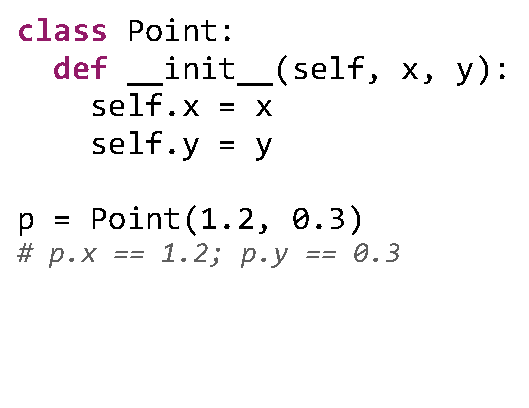
\includegraphics[scale=.55]{figures/python-class-point-code}
  \label{fig:ch5-python-class-point-code}
}
\subfigure[Generated Java class for \texttt{Point}]{
  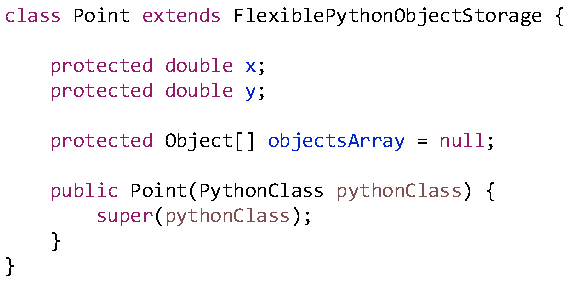
\includegraphics[scale=.8]{figures/flexible-object-storage-class-point-code}
  \label{fig:ch5-flexible-object-storage-class-point-code}
}
\caption{Flexible object storage example}
\label{fig:ch5-flexible-object-storage-example-code}
\end{figure}

In addition to the fixed object storage, ZipPy also uses a class file generation based approach to produce unique object storages for each Python class at runtime.
Figure~\ref{fig:ch5-flexible-object-storage-example-code} gives an example of the generated object storage.
As shown in Figure~\ref{fig:ch5-python-class-point-code}, the simple Python class \texttt{Point} only has two attributes, \texttt{x} and \texttt{y}.
The instantiation of \texttt{Point} shown in the Figure assigns two doubles to \texttt{x} and \texttt{y}.
Based on this type information, ZipPy generates the Java class \texttt{Point} shown in Figure~\ref{fig:ch5-flexible-object-storage-class-point-code} as the object storage for instances of the Python class.
Note that the generated Java class has two double fields to store the attributes of the Python class.
We generate the object storage class optimistically assuming that the layout of a Python \texttt{Point} object does not change in the future and the types of its attributes are also stable.
If our assumption holds, the generated Java class is the optimal object storage tailored specifically for the Python class \texttt{Point}.
In case of a layout change such as adding a new attribute or an attribute type change, the generated object storage will utilize the spill array as the fall back to accommodate new attributes.
Upon the removal of an attribute, we simply remove it from the layout table and leave the freed object storage location un-utilized.

The above mentioned object storage generation relies on layout information collected in the instantiation of the Python class.
We do not have enough information about the object layout ahead of time or before the first instantiation of the Python class at runtime.
On the other hand delaying the object storage generation results in diminishing returns, since a large number of Python objects allocated before hand cannot benefit from this optimization.
Therefore the most effective way is to generate a flexible object storage for the Python class when it first instantiated.
ZipPy uses a specialized constructor call node to perform the first instantiation of a Python class in the following steps:

\begin{enumerate}

\item Create a fixed object storage, which we refer as a bootstrapping object, to collect layout information from the constructor call.

\item Call the resolved constructor, and pass the bootstrapping object as the first argument \textsf{self}.

\item After the constructor call, generate a flexible object storage class based on the current layout of the bootstrapping object similar to the one shown in Figure~\ref{fig:ch5-flexible-object-storage-class-point-code}.

\item Create a flexible object storage using the generated storage class, and migrate the attributes from the populated bootstrapping object to the flexible object storage.

\item Rewrite the constructor call node to a version that optimizes the subsequent constructor calls by directly allocating a flexible object storage.

\item Invalidate the layout on the fixed object storage and return the instantiated flexible object storage to the caller.

\end{enumerate}

Even though we rely on a fixed object storage to bootstrap the class generation, we discard it immediately after migrating all the attributes to the flexible object storage.
Therefore, the caller of the Python constructor does not hold reference to the bootstrapping object, and it is in most cases safe to ignore it.
However, there is a special case where the bootstrapping object is accessed again.
We will discuss this issue in more detail in Section~\ref{sec:ch5-zombie-resurrection}.

Note that the bootstrapping process described above only happens once for each Python class.
After the successful generation of the flexible storage class, any subsequent attempt to instantiate the same Python class automatically picks up the updated storage class.
If the Python program does not instantiate a loaded Python class, ZipPy does not generate flexible storage class for it.

\subsection{Continuous Storage Class Generation}
\label{sec:ch5-flexible-storage-layout-evolution}

\begin{figure}
\centering
\subfigure[Extended Python class \texttt{Point}]{
  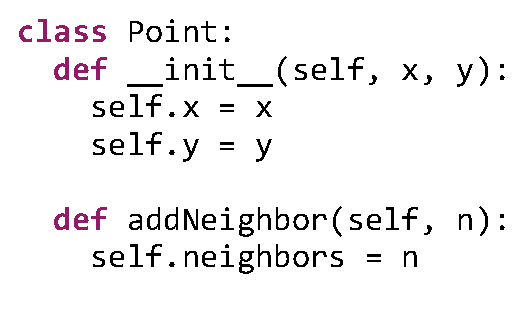
\includegraphics[scale=.6]{figures/python-class-point-with-layout-change-code}
  \label{fig:ch5-python-class-point-with-layout-changecode}
}
\subfigure[A loop that uses the \texttt{Point} class]{
  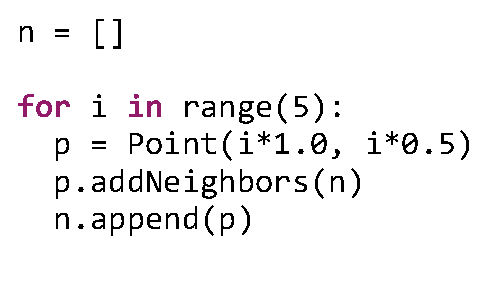
\includegraphics[scale=.6]{figures/python-class-point-used-in-loop-code}
  \label{fig:ch5-python-class-point-used-in-loop-code}
}
\caption{Python object layout change example}
\label{fig:ch5-python-object-layout-change-example-code}
\end{figure}

The above mentioned flexible object storage generation rely on a common practice among Python programmers that is do not abuse the mutability of Python objects after its instantiation.
Since it is permitted by the language, a large portion of Python programs do not strictly follow this practice.
Figure~\ref{fig:ch5-python-object-layout-change-example-code} shows an updated implementation of the Python class \texttt{Point} that changes its object layout outside the constructor.
Note that the new implementation has an additional method called \texttt{addNeighbors}.
The method inserts a new attribute to the instances of \texttt{Point}.
A hypothetical loop shown in Figure~\ref{fig:ch5-python-class-point-used-in-loop-code} calls the \texttt{addNeighbors} method in the loop body, and causes a layout change after the instantiation of the class \texttt{Point}.
The behavior of the program shown in the Figure does not follow the suggested coding practice, however, it is in fact commonplace among Python programs.

Although flexible object storage is capable of handling layout changes like the one shown in Figure~\ref{fig:ch5-python-object-layout-change-example-code}, it does so by spilling the new attribute to the spill array.
A few number of layout changes occurred after the instantiation is enough to cripple the performance advantage of using such a flexible object storage.
To address this issue we extended flexible object storage generation in ZipPy to support continuous generation of storage classes.
Every newly generated storage class adopts the layout changes happened so far.
So if the layout changes converge to a stable point, ZipPy allocates all subsequently instantiated Python objects using the optimal flexible object storage.

\begin{figure}
\centering
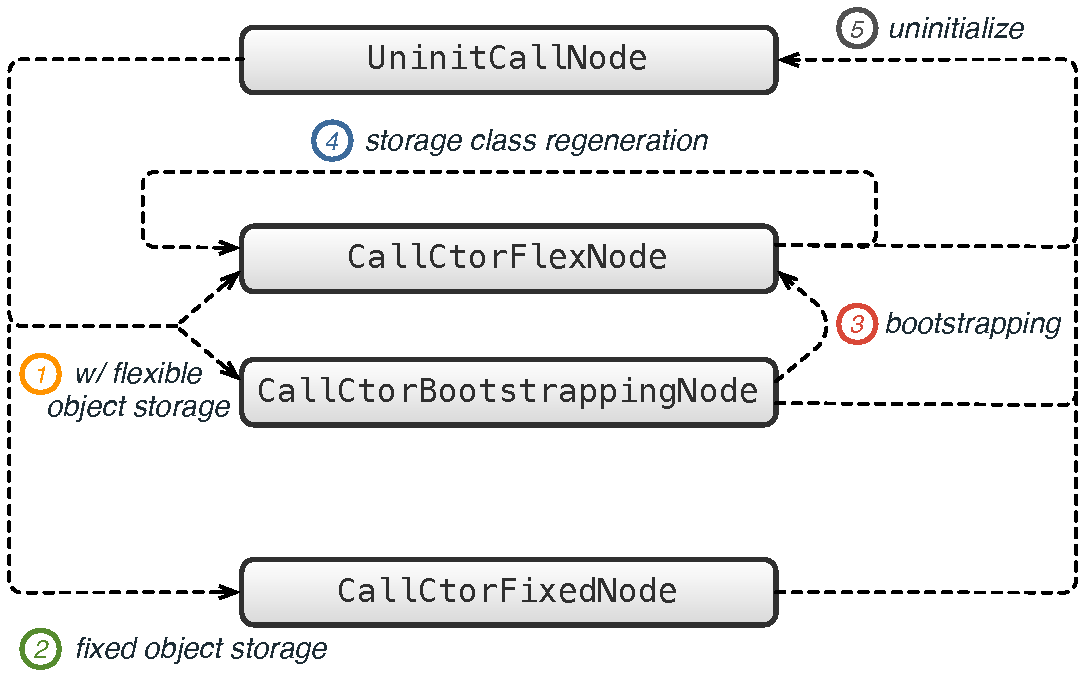
\includegraphics[scale=.45]{figures/constructor-call-site-transformation}
\caption{Constructor call site transformation}
\label{fig:ch5-constructor-call-site-transformation}
\end{figure}

ZipPy supports continuous storage class generation by applying a series of node transformations on a constructor call site.
We implement a number of call node versions specifically for constructor calls or constructor call nodes.
Each version handles the allocation of the new Python object in a different way.
Figure~\ref{fig:ch5-constructor-call-site-transformation} shows the various call constructor nodes in ZipPy.
The descriptions of each node is as follows:

\begin{itemize}

\item \texttt{UninitCallNode}: Uninitialized call node representing an un-executed call site.

\item \texttt{CallCtorFlexNode}: Specialized constructor call node that allocates Python object instances using a flexible object storage.

\item \texttt{CallCtorBootstrappingNode}: Specialized constructor call node that bootstraps the initial flexible storage class generation.

\item \texttt{CallCtorFixedNode}: Specialized constructor call node that allocates Python object instances using a fixed object storage.

\end{itemize}

Figure~\ref{fig:ch5-constructor-call-site-transformation} also illustrates the transformations between different call constructor nodes that enables continuous storage class generation.
The descriptions of the transformation rules are as follows:

\begin{enumerate}

\item With flexible object storage enabled, upon the first execution of a constructor call site, ZipPy rewrites the uninitialized call node to a constructor call node that allocates flexible object storages.
If this call is the first instantiation of the target Python class, we rewrite the call node to a \texttt{CallCtorBootstrappingNode}.
Otherwise, if the target Python class has an existing flexible storage class, we rewrite the call node to a \texttt{CallCtorFlexNode}.

\item With flexible object storage disabled, the initialization of a constructor call site rewrites the call node simply to a \texttt{CallCtorFixedNode}.

\item After the first instantiation of a Python class, the \texttt{Call-\\CtorBootstrappingNode} generates the first flexible storage class and rewrites itself to a \texttt{CallCtorFlexNode}.

\item When a \texttt{CallCtorFlexNode} detects a layout change, it generates an updated Java storage class for the target Python class, and allocates a Python object using the updated storage class.
It also rewrites itself to a new \texttt{CallCtorFlexNode} optimizing for the allocation of the updated storage class.

\item If the callee of the constructor call changes, all specialized call node transforms back to the uninitialized call node.

\end{enumerate}

Each Python class keeps track of its own Java storage classes used to instantiate the Python class.
It marks the most recently generated storage class as its current storage class.
Each \texttt{CallCtorFlexNode} caches the current storage class and the Java method handle~\cite{jdk8} of its constructor.
When allocating an object storage, the \texttt{CallCtorFlexNode} calls the Java constructor of the storage class by using the cached method handle.
A Python object layout change signals its Python class to mark the current storage class as ``old''.
The following instantiation of the Python class triggers an storage class generation, and replaces the ``old'' current storage class with the ``new'' one.
Subsequent instantiations of the Python class automatically pick up the update, and make sure to allocate Python object instances using the current storage class.

\subsection{A Generalization to the Object Model}

\begin{figure*}
\centering
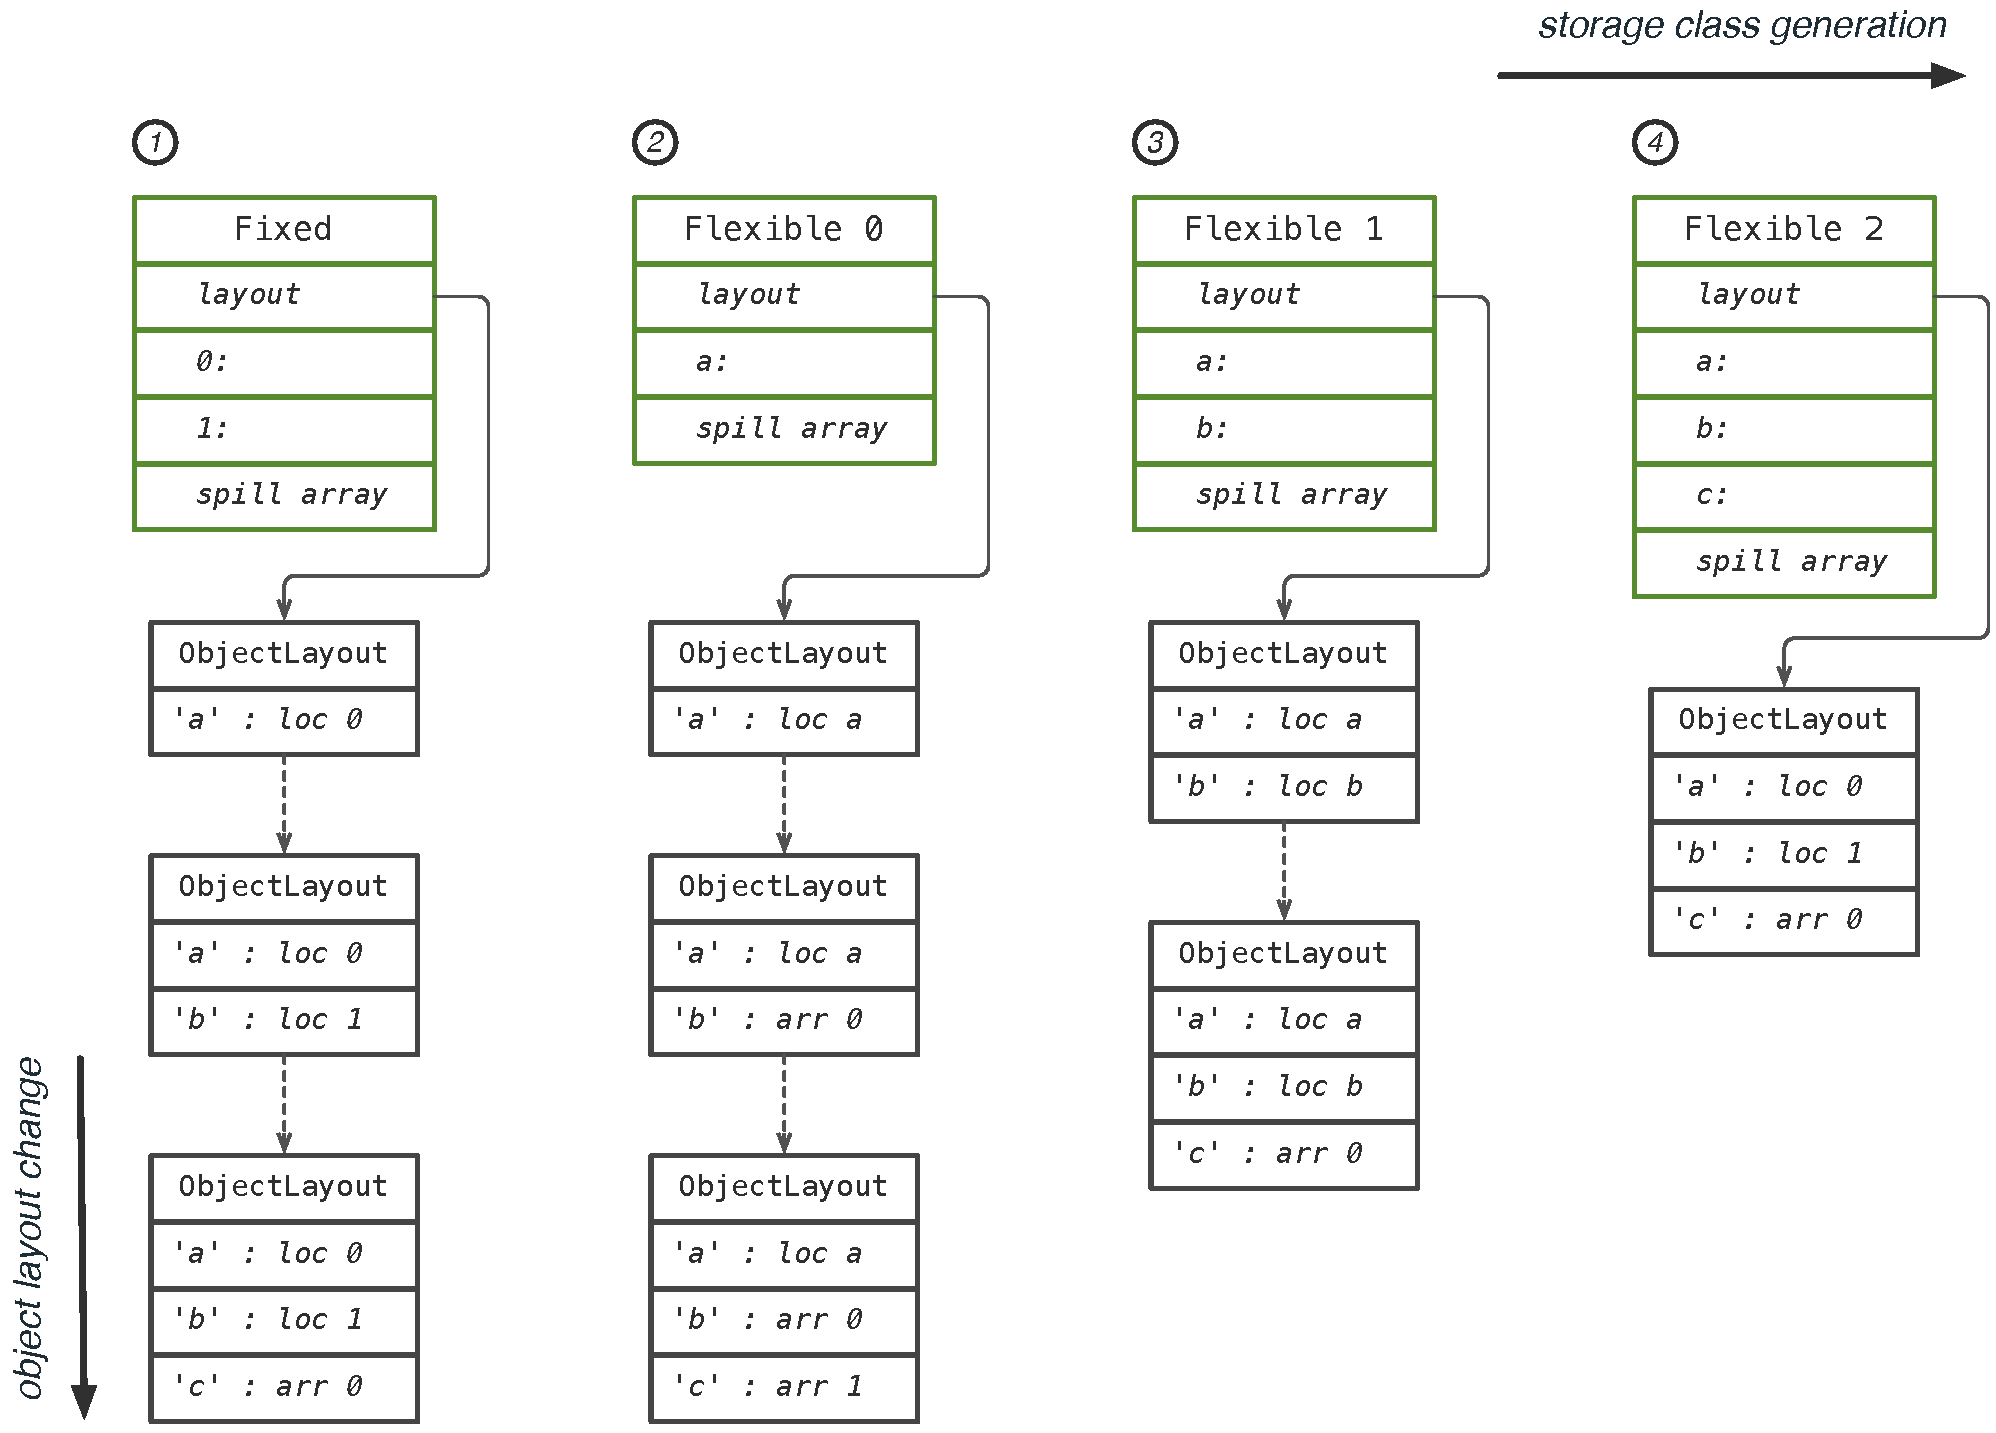
\includegraphics[scale=.49]{figures/object-storage-class-generation-and-object-layout-change}
\caption{Continuous storage class generations and object layout changes of an example Python class}
\label{fig:ch5-object-storage-class-generation-and-object-layout-change}
\end{figure*}

Continuous storage class generation generalizes the existing object model of ZipPy to enable the use of multiple storage classes for a single Python class.
Figure~\ref{fig:ch5-object-storage-class-generation-and-object-layout-change} illustrates the transitions of storage classes and object layouts of an example Python class during the life time of the class.
In the object model described previously where we only use fixed storage classes to model Python objects, an object layout change at runtime triggers a transition vertically in the Figure.
Whereas with continuous storage class generation an object layout change also triggers a storage class regeneration along the horizontal direction in the Figure.
The transitions of the storage classes are orthogonal to that of the object layouts.
Each storage class follows its own object layout transitions.

Every Python object has its own life time.
The life time starts from the instantiation of the object, and ends at the point that it is not referenced by the program and ready to be garbage collected.
In the middle of its life time, a Python object allocated using on storage class in general cannot migrate its attributes to use another storage class.
Since there could be existing pointers that reference the current object storage of the Python object, a storage class migration will turn those existing pointers into dangling pointers.
Therefore, a Python object needs to reside in a single object storage throughout its life time.

A storage class generation caused by an object layout change only benefits Python objects instantiated after the layout change.
The living or existing objects of the same Python class handle layout changes lazily by spilling the new attribute to the spill array and updating its own layout table.
Note that similar to the fixed object layout approach, we synchronize object layout changes across all the Python objects allocated using the same storage class.
We will use a program execution example to further explain the object layout synchronizations.
For instance, along the execution of a hypothetical Python program, the program at one point allocates two Python object \textsf{A} and \textsf{B} both using the storage class \texttt{Flexible 0} shown in Figure~\ref{fig:ch5-object-storage-class-generation-and-object-layout-change}.
Since Python object instantiation always picks up the latest storage class, \texttt{Flexible 0} is the most current storage class at this point.
Both \textsf{A} and \textsf{B} only have a single attribute \texttt{a}.
At a later point, an object layout takes place by adding an attribute \texttt{b} to the object \textsf{A}.
Object \textsf{A} updates its own layout table, invalidates the previous object layout, and sets the new object layout as the valid layout of \texttt{Flexible 0}.
Since we invalidated the previous object layout, any object that still uses the old layout needs to \emph{synchronize} to the updated layout.
The following access to object \textsf{B} will cause an slow path execution that synchronizes its object layout with \texttt{Flexible 0}.
After the layout synchronization, even though object \textsf{B} does not actually contain the attribute \texttt{b}, its layout table includes an entry for \texttt{b}.
Note that the above mentioned layout change also signals the Python class to generate storage class \texttt{Flexible 1}.
However, object \textsf{A} and \textsf{B} will not migrate to another storage class and always synchronize its with \texttt{Flexible 0} to share the same object layout.

Object layout synchronization simplifies the attribute access dispatch we explained in Section~\ref{sec:ch5-attribute-access-dispatch-chain}.
It ensures that we only need to maintain a single valid cache entry to access Python objects allocated using the same storage class.
However, in its life time, a Python class could generate multiple storage classes.
It is inevitable that at the same program location we need to built multiple cache entries, one for each storage class, to optimize accesses to Python objects of the same class.

\subsection{Zombie Resurrection}
\label{sec:ch5-zombie-resurrection}

\begin{figure}
\centering
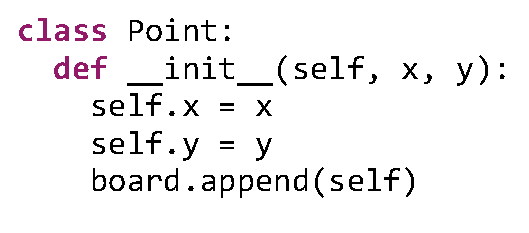
\includegraphics[scale=.6]{figures/python-class-point-with-zombie-store-code}
\caption{A Python constructor that exposes a reference to \texttt{self}}
\label{fig:ch5-python-class-point-with-zombie-store-code}
\end{figure}

We uses a fixed object storage to bootstrap the initial storage class generation.
But we only return the instantiated Python object to the caller of the constructor after migrating to a flexible object storage and discarding the initial fixed one.
This approach ensures that the consumer of the constructor call only references the flexible object storage.
However, there are cases where the constructor itself could expose the reference to the fixed object storage making it accessible outside the constructor.
Figure~\ref{fig:ch5-python-class-point-with-zombie-store-code} shows a modified definition of the Python class \texttt{Point}.
The constructor of \texttt{Point} stores a reference to \texttt{self} to the Python list \texttt{board}.
The reference store makes potential accesses to \texttt{self} possible outside the constructor.
So during the storage class bootstrapping of \texttt{Point}, the shown reference store of \texttt{self} will make the bootstrapping object modeled using the fixed object storage accessible at a later point.
We refer this scenario as zombie resurrection.
Since the bootstrapping object, in most case a \emph{dead} object, comes to live again in this particular situation.

We address this issue by turning the zombie object storage into a proxy to the flexible storage object it migrates to.
To be more specific, in the last step of bootstrapping a storage class generation, after migrating to the flexible object storage, we pass a reference to the flexible object storage the zombie object storage, and flag it as a proxy.
As a proxy, the zombie redirects all attribute accesses to the flexible object storage.
This approach ensures that all references to the first instance of a Python class eventually access the same flexible object storage, hence, preserves the correct semantics.

\subsection{Discussion}

ZipPy execute Python programs first in the interpreter mode, and compiles the program when it becomes hot.
The warming up phase of the guest program executes in interpreter mode.
ZipPy compiles the Python program only after it has been executed for a few iterations when the specializations of the program become stable.
The same type locality principle applies to Python object layouts as well.
That is the layouts of Python objects of the same class tend to converge and stabilize after the initial warm up phase.
Therefore, ZipPy in most cases compiles Python programs only after their object layout evolution has stabilized.
The underlying Java JIT compiler treats Python objects as regular Java objects, since we model them using ordinary Java objects.
The compiler is able to apply aggressive optimizations such as escape analysis to Python objects as well.
When combined with flexible storage class generation, our object model design offers both performance and space efficiency that closes the gap between the guest language and the host language.

\section{Evalutation}

To fully assess the effectiveness of the optimizations we discussed in the Chapter~\ref{chp:ch6-object}, we evaluate the performance of ZipPy in the following steps:
First we evaluate the overall performance of ZipPy by running a selection of conventional benchmarks.
These benchmarks are popular among the virtual machine research and Python communities.
They provide a good indication of the overall performance of a programming language implementation.
Second we examine the effectiveness of generator peeling using a set of real world and generator intensive Python programs.
As the last step, we analyze the performance and space impact of using flexible object storage generation in ZipPy.
We organize our extensive performance experiments by comparing ZipPy with the existing Python VMs.

\section{The Performance of ZipPy}
\label{sec:ch6-performance-of-zippy}

\subsection{Experiment Setup}

We evaluate the overall performance of ZipPy by comparing the performance of our system with existing Python VMs, such as CPython~\cite{python}, Jython~\cite{jython} and PyPy~\cite{pypy}.
Our system setup is as follows:

\begin{itemize}

\item Intel Xeon E5462 Quad-Core processor running at a frequency of 2.8GHz, on Mac OS X version 10.9.3 build 13D65.

\item Apple LLVM 5.1, OpenJDK 1.8.0\_05, Truffle/Graal 0.3.\footnote{From source code repository \url{http://hg.openjdk.java.net/graal/graal}}

\end{itemize}

The VM versions used in the comparison and the description of their execution models are as follows:

\begin{itemize}

\item CPython 2.7.6 and 3.4.0: Interpreter only.

\item Jython 2.7-beta2:
Python 2 compliant, hosted on JVMs.
Compiles Python modules to Java classes and lets the JVM JIT compiler further compiles them to machine code.

\item PyPy 2.3.1 and PyPy3 2.3.1: Python 2 and 3 compliant respectively.
Uses a meta-tracing JIT compiler that compiles Python code to machine code.

\end{itemize}

% Python 2 vs. Python 3
Python 3 is not backward compatible with Python 2.
Although ZipPy exclusively supports Python 3, including well-established Python 2 VMs in the comparison highlights the potential of our optimization.
The benchmarks we chose support both Python 2 and 3.
The same code, however, suffers from a slight difference in the semantics interpreted by different VMs.

% how we measure, peak performance
We run each benchmark ten times on each VM and average the execution times.
For VMs that use a tiered execution strategy, we warm up the benchmarks to ensure that the code is just-in-time compiled.
This allows us to properly measure peak performance.

\subsection{Benchmark Selection}

\begin{table*}
  \begin{center}
    \begin{tabular}{ l l }
    \toprule
    Benchmark suite & Included benchmarks \\
    \midrule
  Computer Language Benchmarks - & \textsf{binarytrees}, \textsf{fannkuchredux}, \textsf{fasta}, \textsf{mandelbrot}, \textsf{meteor} \\
  Games & \textsf{nbody}, \textsf{pidigits}, \textsf{spectralnorm} \\
  \midrule
  Unladen Swallow Benchmarks &  \textsf{float}, \textsf{richards} \\
  \midrule
  PyPy Benchmarks & \textsf{chaos}, \textsf{deltablue}, \textsf{go} \\
    \bottomrule
  \end{tabular}
    \caption{Benchmarks selection}
    \label{tab:ch6-regular-benchmark-selection}
  \end{center}
\end{table*}

We selected a number of benchmarks for the performance experiments from three popular benchmark suites.
The descriptions of the chosen benchmark suites are as follows:

\begin{itemize}

\item Computer Language Benchmarks Game~\cite{benchmarkgame}: a popular benchmark suite for evaluating and comparing the performance of different programming languages.

\item Unladen Swallow Benchmarks~\cite{unladen.swallow}: the benchmark suite used by the unladen swallow project.
Unladen swallow is an optimization branch of CPython built by Google.
The goal of the project was to become a faster yet fully compatible modification of CPython.
Its benchmark suite is well-regarded in the Python community.

\item PyPy Benchmarks: a collection of benchmarks used by the PyPy project.

\end{itemize}

Table~\ref{tab:ch6-regular-benchmark-selection} summarizes the benchmarks we selected in this experiment from the above mentioned suites.
Since we focus on the overall performance of Python VMs, we intentionally leave out benchmarks that are sensitive to the performance of generators.
We selected benchmarks that are written in both imperative and object oriented styles.

\subsection{Experiment Results}

\begin{table*}
  \small
  \begin{center}
  \begin{tabular}{ l r r r r r r }
  \toprule
  Benchmark     & CPython3  & CPython  & Jython  & PyPy     & PyPy3    & ZipPy \\
  \midrule
  \textsf{binarytrees}   & $5.40$    & $5.10$   & $10.76$ & $14.05$  & $14.60$  & $39.49$ \\
  \textsf{fannkuchredux} & $2.27$    & $2.20$   & $1.17$  & $101.24$ & $107.52$ & $198.94$ \\
  \textsf{fasta}         & $15.52$   & $16.20$  & $24.13$ & $182.09$ & $174.55$ & $241.76$ \\
  \textsf{mandelbrot}    & $9.00$    & $9.70$   & $3.03$  & $98.15$  & $97.35$  & $105.18$ \\
  \textsf{meteor}        & $100.55$  & $102.83$ & $77.14$ & $265.43$ & $263.75$ & $213.77$ \\
  \textsf{nbody}         & $10.12$   & $9.87$   & $7.40$  & $122.83$ & $122.07$ & $62.42$ \\
  \textsf{pidigits}      & $77.02$   & $77.40$  & $47.59$ & $75.25$  & $73.02$  & $46.59$ \\
  \textsf{spectralnorm}  & $0.90$    & $1.20$   & $1.70$  & $114.60$ & $114.52$ & $115.29$ \\
  \textsf{float}         & $10.82$   & $10.23$  & $11.37$ & $93.57$  & $93.82$  & $191.68$ \\
  \textsf{richards}      & $16.77$   & $15.83$  & $20.35$ & $495.38$ & $490.70$ & $840.93$ \\
  \textsf{chaos}         & $2.05$    & $2.40$   & $3.17$  & $83.77$  & $52.65$  & $139.94$ \\
  \textsf{deltablue}     & $19.62$   & $16.77$  & $26.19$ & $590.25$ & $571.82$ & $460.37$ \\
  \textsf{go}            & $23.15$   & $24.97$  & $46.16$ & $157.29$ & $154.07$ & $356.80$ \\
  \bottomrule
  \end{tabular}
  \caption{The scores of Python VMs running regular benchmarks}
  \label{tab:ch6-regular-benchmarks-scores}
  \end{center}
\end{table*}

\begin{table*}
  \small
  \begin{center}
  \begin{tabular}{ l r r r r r r }
  \toprule
  Benchmark     & CPython3  & CPython  & Jython  & PyPy     & PyPy3    & ZipPy \\
  \midrule
  \textsf{binarytrees}   & $1.00$    & $0.94$   & $1.99$  & $2.60$   & $2.70$   & $7.31$ \\
  \textsf{fannkuchredux} & $1.00$    & $0.97$   & $0.51$  & $44.53$  & $47.29$  & $87.50$ \\
  \textsf{fasta}         & $1.00$    & $1.04$   & $1.55$  & $11.73$  & $11.24$  & $15.57$ \\
  \textsf{mandelbrot}    & $1.00$    & $1.08$   & $0.34$  & $10.91$  & $10.82$  & $11.69$ \\
  \textsf{meteor}        & $1.00$    & $1.02$   & $0.77$  & $2.64$   & $2.62$   & $2.13$ \\
  \textsf{nbody}         & $1.00$    & $0.97$   & $0.73$  & $12.13$  & $12.06$  & $6.17$ \\
  \textsf{pidigits}      & $1.00$    & $1.00$   & $0.62$  & $0.98$   & $0.95$   & $0.60$ \\
  \textsf{spectralnorm}  & $1.00$    & $1.33$   & $1.89$  & $127.33$ & $127.25$ & $128.10$ \\
  \textsf{float}         & $1.00$    & $0.95$   & $1.05$  & $8.64$   & $8.67$   & $17.71$ \\
  \textsf{richards}      & $1.00$    & $0.94$   & $1.21$  & $29.53$  & $29.25$  & $50.13$ \\
  \textsf{chaos}         & $1.00$    & $1.17$   & $1.55$  & $40.88$  & $25.69$  & $68.28$ \\
  \textsf{deltablue}     & $1.00$    & $0.85$   & $1.33$  & $30.08$  & $29.14$  & $23.46$ \\
  \textsf{go}            & $1.00$    & $1.08$   & $1.99$  & $6.79$   & $6.66$   & $15.41$ \\
  \textbf{mean}          & \textbf{1.00}    & \textbf{1.02}   & \textbf{1.05}  & \textbf{12.15}  & \textbf{11.68}  & \textbf{15.34} \\
  \bottomrule
  \end{tabular}
  \caption{The speedups of Python VMs normalized to CPython3 running regular benchmarks}
  \label{tab:ch6-regular-benchmarks-speedups}
  \end{center}
\end{table*}

Table~\ref{tab:ch6-regular-benchmarks-scores} and~\ref{tab:ch6-regular-benchmarks-speedups} shows the results of our experiments.
We use a score system to gauge VM performance.
We calculate the score by dividing $1000$ by the execution time of the benchmark.
A score system is more intuitive than execution times for visualization purpose.
It also offers a higher resolution for our performance measurements.
We carefully chose the program inputs such that the resulting scores stay in the range between $10$ and $1000$.
Larger inputs have limited impacts on the speedups our of optimization.

Table~\ref{tab:ch6-regular-benchmarks-scores} shows the average scores of each Python VM running the selected benchmarks.
Table~\ref{tab:ch6-regular-benchmarks-speedups} shows the average speedups of each VM against CPython3.
We calculate the speedups by normalizing the scores of each VM shown in Table~\ref{tab:ch6-regular-benchmarks-scores} against that of CPython3.
The last row of Table~\ref{tab:ch6-regular-benchmarks-speedups} shows the geometric mean of the speedups of each Python VM relative to CPython3.
As shown in the Table, the average speedup of ZipPy over CPython3 is $\zippyToCPythonRegular{}\times$ with the highest speedup over $128\times$ on \textsf{spectralnorm}.
Note that the performance of ZipPy running the selected benchmarks is even higher than PyPy by around $26\%$

\subsection{Performance Analysis}

The majority of the high number speedups of ZipPy comes from compute intensive benchmarks like the ones from the Computer Language Benchmarks Game.
The unboxed data representation of numeric types in ZipPy successfully optimizes these benchmarks without ever having to go to the boxed representation.
At peak performance, ZipPy executes the entire benchmark by only using Java primitives for arithmetic operations.
This approach effectively enables low level optimizations offered by the underlying Graal compiler, which consequently achieved Java like arithmetics performance for Python programs in our experiments.
Being able to speculatively reduce the cost of arithmetic operations in Python to be much closer to that in Java is the key distinguisher between ZipPy and the existing JVM-based Python implementations.

The noticeable slow down in \textsf{pidigits} is caused by integer overflows in Python.
After an integer overflow, ZipPy uses a JDK \texttt{BigInteger}~\cite{hotspot} to model integers of a large value.
However, the implementation of \texttt{BigInteger} in the JDK did not outperform the implementation of \texttt{PyInt} in CPython on our benchmark.
We did not pursue in the direction of replacing \texttt{BigInteger} with a more efficient alternative written in Java, since we consider the implementation details of an unbound integer type to be orthogonal to the research we discuss in this thesis.

We also see speedups of multiple of $10\times$ on object-bound benchmarks like \textsf{richards} and \textsf{chaos}.
We only use fixed object storages in this experiment.
The results suggest that the Python object model used in ZipPy is orders of magnitude more efficient that the hash map based ones used in CPython and Jython.
The object layout based approach in ZipPy clears the way on letting the underlying Java compiler to optimize Python object accesses the same way as it does to Java objects.
In the common case where the object layouts stabilize shortly after warming up, ZipPy essentially delivers Java like performance on Python object operations in our experiment.

Overall ZipPy outperforms PyPy in our experiment.
We attribute this advancement to Graal, the underlying Java JIT compiler.
PyPy uses a relatively straight forward tracing JIT compiler to compile Python programs down to machine code.
Whereas Graal is a substantially more sophisticated and aggressive method JIT.
The kinds of optimizations implemented in Graal outnumbered that in PyPy.
Overall we do expect Graal to generate more efficient machine code than the compiler in PyPy.

In general the speedups we achieved in our experiment are inline with other efficient Truffle language implementations~\cite{seaton2014debugging,Grimmer+2014,Grimmer+2014TruffleC}.
A number of semi built-in optimizations offered by Truffle helped us achieving this result.
The most important ones includes: frame optimization that eliminates the heap allocation of a frame object and Truffle AST inlining.
Another advantage of using Truffle as the base of ZipPy is that it makes it easy for guest language implementers to fine tune the machine code size produced by the compiler.
Truffle offers utilities that helps us to precisely specify the boundary of a JIT compilation rather than fully relying on the compiler heuristics.
This features allows us to carve out less important code paths from the compiled code to make the machine code size more compact.
In summary, by making better use of Truffle ZipPy is able to achieve high speedups when compared with existing Python VMs with low implementation cost.

\section{The Effectiveness of Flexible Object Storages}

In the overall performance evaluation of ZipPy we used a fixed object storage configuration in our experiments.
Here we extend our experiments and evaluates the implementation of flexible object storage in ZipPy.
We do so by comparing the time and space efficiency between the different object model configurations in ZipPy.
We select a number of object-bound benchmarks from our comprehensive benchmark selection for this particular experiments.
Those benchmarks includes: \textsf{float}, \textsf{richards}, \textsf{chaos}, \textsf{deltablue} and \textsf{go}.
We used the same experiment setup as mentioned previously in Section~\ref{sec:ch6-performance-of-zippy}.

\subsection{Object Model Configurations}

As we discussed in Chapter~\ref{chp:ch6-object}, a fixed object storage has a fixed number of fields to stores Python object attributes.
To accommodate attributes modeled using Java primitive types, a fixed object storage needs to have fields of different types, such as Java \textsf{int}, \textsf{double} and \textsf{Object}.
In our experiment, we use fixed object storages that have equal number of fields of each of these three types.
Note that we cannot mix the fields of different types, since the binary representation of each type varies in different JVM implementations.
For instance, some versions of the HotSpot VM~\cite{hotspot} use a technique called pointer compression to reduce the size of a Java object pointer.
Therefore, storing a non-pointer value in a pointer field using \textsf{Unsafe} will lead to unexpected behavior at runtime.
The size of a fixed object storage refers to the number of fields of each type the storage has.
The bigger the storage size the more attribute it can accommodate in a field.
However, larger storage size also lead to memory space inefficiency.
Since a large portion of the object storage space maybe not be utilized.
In the overall performance evaluation, the space configuration of the fixed object storage used in ZipPy is five.

The size of a flexible object storage is determined at runtime.
The two different configurations we used in our experiment are \emph{simple flexible object storage} and \emph{flexible object storage with continuous generation}.
Simple flexible object storage means we only generate one storage class for each Python class.
We handle all post-constructor object layout change by using the spill array.
In flexible object storage with continuous generation, we always generate a new storage class whenever a layout change takes place.

\subsection{The Performance of Flexible Object Storages}

\begin{figure*}
\centering
\includegraphics[scale=.3, page=4]{benchmarks/object-model-results}
\caption{Detailed speedups of different object model configurations normalized to fixed object storage of size $5$}
\label{fig:ch6-object-model-config-speedup}
\end{figure*}

Figure~\ref{fig:ch6-object-model-config-speedup} shows the performance of each object model configuration running the selected benchmarks normalized to the fixed object storage.
With flexible object storage enabled we discover speedups when running the majority of the benchmarks with the highest speedup of $14\%$ on \textsf{chaos}.
The average speedup of using flexible object storage is $2$ to $3\%$.
We also notice a slowdown on \textsf{richards}.
The worse case slowdown caused by using flexible object storage is about $22\%$.

We did not observe more aggressive speedups, because of the high setting on the size of the baseline fixed object storage configuration.
A fixed object storage of size five has fifteen fields.
Given that most Python objects allocated at runtime are small in size, a fixed object storage of size five is in most cases more than enough to accommodate all the attributes of a Python object.
Having a high setting on the size of fixed object storage enables better performance but at the price of allocating more space for each Python object.

Flexible object storage on the other hand ensures that we allocate just enough memory space for a Python object.
Continuous storage class generation also guarantees that any new object allocation is performance wise optimal based on the latest layout description of the object.
On a few benchmarks enabling continuous storage class generation causes a moderate slowdown.
This slowdown is caused by higher degree of polymorphism potentially introduced by new storage class generation at an object access site.
After the generation of a new storage class, the Python object instances allocated using an old storage class might still be alive.
The mix of storage classes causes the access of Python objects of the same Python class to use multiple inline cache entries.
The increase in the number of cache entries leads to a slowdown that we observed in our results.
The more noticeable slowdown on \textsf{richards} when enabling flexible object storage is due to the current implementation of Truffle we used in this experiment.
Switching the object storage configuration causes a change in the AST inlining pattern for \textsf{richards}.
As a consequence, this pattern change results in a slowdown in our experiment.
We expect that using a newer version of Truffle with updated inlining heuristics will correct this fluctuation.

A fixed object storage configuration is always biased.
A single size configuration cannot work well for all Python programs let alone the fixed type distribute among the fields of an object storage.
Even with a high size setting, using fixed object storage is $14\%$ slower than the flexible approach as shown in Figure~\ref{fig:ch6-object-model-config-speedup}.
The reason behind is the allocation of large Python objects.
Any attribute that cannot fit into the fixed object storage is stored in the spill array.
The additional memory access incurred by accessing the spill array causes a slowdown on the benchmark.

\subsection{The Space Efficiency of Flexible Object Storages}

\begin{figure}
\centering
\includegraphics[scale=.27, page=5]{benchmarks/object-model-results}
\caption{The memory overheads of fixed object storage of size $1$, $3$ and $5$ relative to flexible storage allocation with continuous generation}
\label{fig:ch6-fixed-object-storage-space-overhead}
\end{figure}

\begin{figure}
\centering
\includegraphics[scale=.27, page=6]{benchmarks/object-model-results}
\caption{The slowdowns of fixed object storage of size $1$, $3$ and $5$ relative to flexible storage allocation with continuous generation}
\label{fig:ch6-fixed-object-storage-slowdown}
\end{figure}

We measured the memory space used to allocate fixed object storages for each selected benchmark with three distinct size settings: one, three and five.
We compare the memory space numbers with the equivalent measured using flexible object storage with continuous generation enabled.
Figure~\ref{fig:ch6-fixed-object-storage-space-overhead} shows the results of this experiment normalized to the memory space usage of flexible object storage.
Using a fixed object storage of size one allocates on average $1.63\times$ more memory than using flexible object storage.
Using a fixed object storage of size five allocates up to $3.6\times$ more memory than using the flexible configuration.

The result shows that using a fixed object storage causes significant memory overhead.
We attribute this inefficiency to the poor type distribution among the fields of a fixed object layout.
In theory one could design an improved solution that generates a library of fixed object storage with various combination of sizes and type distributions ahead of time, and pick the closest fit from the library when allocating a Python object.
Since flexible object storage ensures the optimal space and type distribution allocated for a given Python object.
This multi-variant fixed object storage solution, even in an ideal case, cannot surpass flexible object storage in terms of space efficiency.

We also measured the slowdown of using a fixed object storage running the benchmarks compared to using flexible object storages.
The fixed object storage configurations used in our experiment includes the following size settings: one, three and five.
Figure~\ref{fig:ch6-fixed-object-storage-slowdown} shows the slowdowns of using various fixed object storages.
Overall we observe slowdowns ranging from $2$ to $20\%$ in the results.
The smaller the fixed object storage size the higher the slowdown.
Using a fixed object storage of size one causes a slowdown up to $20\%$ on \textsf{chaos}.
By increase the size of fixed object storages the slowdowns tend to decrease or even diminish.

\subsection{Discussion}

There is always a trade-off when using fixed object storage.
Empirically it is impossible to find an optimal fixed object storage size that offers both space efficiency and performance.
One can either trade memory space for performance, by choosing a bigger fixed object storage size,
or inversely use a smaller size to save memory space at the price of a lower performance.
In our experiments, using fixed object storage either increases memory usage by $3.6\times$, or shows a $20\%$ performance loss.

Flexible object storage, on the other hand, ensures minimum memory usage with optimal performance for each Python class.
Our technique produces a storage class that is optimal in terms of both space and performance for the current status of the Python class.
As the program state evolves over time, our system automatically adapts to the change and generates an updated storage class.

However, continuous flexible storage class generation can lead to multiple storage classes coexisting for a single Python class.
These generated storage classes incurs a small memory overhead.
This overhead is, however, negligible when compared to the memory allocated for Python instance objects.
Multiple storage classes also create multiple valid cache entries in an object access inline cache.
These additional cache entries cause the slowdown in \textsf{richards} when compared to a fixed object storage of size $5$.
Given that the memory usage significantly overweights the speed loss for \textsf{richards} of size $5$, we think flexible object storage still delivers a much better balance between space and performance than its fixed counterpart even in the worst case of our tests.

Furthermore, ZipPy can potentially alleviate this slowdown by carefully reordering the cache entries created for the same Python class.
The reordering can hoist the cache entry created for the newer generation storage class above the entries created for the older ones assuming more frequent accesses on the Python objects allocated using the newer storage class.
However, we found in our tests that the benefit of this optimization is input dependent or program behavior dependent.
Some programs access the older storage classes more often, whereas the other programs tend to access the newer ones.
Thus, in our experiments, the benefit of using cache entry reordering is inconclusive.

\section{Conclusions}
This paragraph will end the body of this sample document.


\begin{acks}
  The authors would like to thank Dr. Yuhua Li for providing the
  matlab code of  the \textit{BEPS} method. 

  The authors would also like to thank the anonymous referees for
  their valuable comments and helpful suggestions. The work is
  supported by the \grantsponsor{GS501100001809}{National Natural
    Science Foundation of
    China}{http://dx.doi.org/10.13039/501100001809} under Grant
  No.:~\grantnum{GS501100001809}{61273304}
  and~\grantnum[http://www.nnsf.cn/youngscientsts]{GS501100001809}{Young
    Scientsts' Support Program}.

\end{acks}


\bibliographystyle{ACM-Reference-Format}
\bibliography{zwei}

\end{document}
